\section{Results}
\label{section:results}

\subsection{What is the main difference between preemptive and cooperative scheduling?}
The main difference between preemptive and cooperative scheduling is that in cooperative scheduling any task could theoretically run forever, another task will only get an opportunity to run when the currently running task yields "of its own free will". However in preemptive scheduling, the scheduler can preempt a task if it sees fit and allow another task to run.

\subsection{What is the difference between vTaskDelay() and vTaskDelayUntil()?}
The main difference between vTaskDelay() and vTaskDelayUntil() is predictability and frequency. vTaskDelay() delays for x number of ticks after having been called, however this does not result in a fixed amount of time, the delay is affected by a number of factors like: preemption, the "route" taken through the code, interrupts and other task activity \cite{VTaskDelay2023}\cite{VTaskDelayUntil2023}. vTaskDelay() is therefor unfit for controlling the periodicity of a task. vTaskDelayUntil() specifies an absolute time, and thus will delay until the fixed specified time. vTaskDelayUntil() is therefor more predictable, reliable and is fit for control of the periodicity of tasks.

\subsection{Design of Assignment 2 (priority inversion).}
This implementation of priority inversion builds on the definition of priority inversion given by Saad Mubeen during lecture RTOS 2\cite{mubeenLectureRTOSII2023}. Priority inversion is not simply a low priority task blocking a high priority task. Priority inversion is when a low priority task initially blocks a high priority task and then a mid priority task preempts the low priority task thus making the blocking time for the high priority task (possibly) unbounded since this situation could possibly extend and cause the delay time to diverge (extend to infinity).

The basic design of the priority inversion implemented for Assignment 2 can be seen in Table \ref{tab:design}.

This implementation uses binary semaphores instead of mutex since FreeRTOS mutex is implemented with priority inheritance. Priority inheritance significantly reduces the likely hood of priority inversion.

\begin{table}[ht]
    \centering
    \resizebox{\columnwidth}{!}{\noindent\begin{tabular}{|l|l|l|l|l|}
    \hline
        \textbf{Task} & \textbf{Priority} & \textbf{Period (s)} & \textbf{Workload time (s)} & \textbf{Uses binary semaphore} \\ \hline
        Task 1 & 1 (Low)  & 11 & 4 & Yes \\ \hline
        Task 2 & 2 (Mid)  & 13 & 4 & No  \\ \hline
        Task 3 & 3 (High) & 6  & 3 & Yes \\ \hline
    \end{tabular}}
    \caption{Basic design of priority inversion for Assignment 2. Note that workload time is a rough estimate in the situation when no preemption occurs.}
    \label{tab:design}
\end{table}

This implementation will cause it's first and guaranteed priority inversion at time 13s during Task 1 first job, Task 2 first job and Task 3 second job, see Figure \ref{fig:scheduler}. At time 11s no task is running and Task 1 will be ready and have it's release time, it will instantly lock the binary semaphore, since it's not currently locked, it will then start it's workload. At time 12s, Task 3 will become ready and preempt Task 1, it will then try to lock the binary semaphore, however it gets blocked since Task 1 has locked the binary semaphore. Task 1 will continue to work until time 13s, Task 2 will preempt Task 1 (since binary semaphores do not have priority inheritance) and start its workload. The system has achieved priority inversion at time 13s and Task 3 will miss it's deadline by 4035 ms.

\begin{figure}[h]
    \centering
    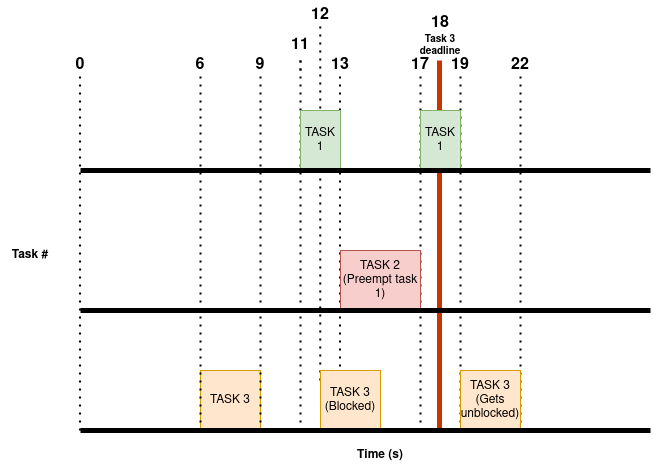
\includegraphics[width=\columnwidth]{images/scheduler.png}
    \caption{Theoretical reenactment of first occurrence of priority inversion.}
    \label{fig:scheduler}
\end{figure}